\chapter{Arhitektura i dizajn sustava}

		\section{Baza podataka}
			
		Za našu platformu koristit ćemo relacijsku bazu podataka. Objekt takve baze je relacija, odnosno tablica koja je definirana svojim imenom i skupom atributa. Atributi unutar jednog entiteta mogu poprimiti funkciju primarnog ili stranog ključa.
Baza podataka ove aplikacije sastoji se od 3 entiteta:
		
			\subsection{Opis tablica}

\noindent \textbf{\textit{profile}}\\
\begin{samepage}
Ovaj entitet sadrži osnovne informacije o korisničkom profilu i  sastoji se od sljedećih atributa: userID (autogenerirani identifikator korisnika) email (email adresa), username (korisničko ime), password(lozinka) name (ime), surname (prezime) i age (dob). UserID je primarni ključ entiteta \textbf{profile}.  
\end{samepage}

    				\begin{longtblr}[
					label=none,
					entry=none
					]{
						width = \textwidth,
						colspec={|X[6,l]|X[6, l]|X[20, l]|}, 
						rowhead = 1,
					} %definicija širine tablice, širine stupaca, poravnanje i broja redaka naslova tablice
     
					\hline \SetCell[c=3]{c}{\textbf{profile}}	 \\ \hline[3pt]
					\SetCell{LightGreen}userID & VARCHAR	&  	jedinstveni identifikator korisnika	\\ \hline
					\SetCell{}email & VARCHAR	&  	jedinstvena e-mail adresa korisnika 	\\ \hline
     				\SetCell{}username & VARCHAR	&  	jedinstveno korisničko ime	\\ \hline
					\SetCell{} password & VARCHAR	&  lozinka korisnika 	\\ \hline
          			\SetCell{} name & VARCHAR	&  ime korisnika (opcionalno)	\\ \hline
               		\SetCell{} surname & VARCHAR	&  	prezime korisnika (opcionalno)	\\ \hline
                    \SetCell{} age & INT	&  	dob korisnika (opcionalno)	\\ \hline
                    
				\end{longtblr}

    
\noindent \textbf{\textit{recipe}}\\
\begin{samepage}
Ovaj entitet opisuje recept postavljen na platformu od strane registriranog korisnika. Primarni je ključ recipeID - (autogenerirani identifikator recepta), a strani ključ userID koji povezuje \textbf{recipe} i \textbf{profile}. Ostali atributi su likes (broj oznaka "sviđa mi se" na receptu od strane registriranih korisnika) koji je inicijalno postavljen na 0, ingredients (sastojci jela koje recept opisuje), name (ime recepta), instructions (niz uputa pripreme jela opisanog receptom), origin (mjesto podrijetla jela), category (kategorija jela), specialTags (dodatne oznake), imageURL (URL slike koju korisnik prilaže uz postavljeni recept) te videoURL (URL videa koji korisnik prilaže uz postavljeni recept).
\end{samepage}
    
    				\begin{longtblr}[
					label=none,
					entry=none
					]{
						width = \textwidth,
						colspec={|X[6,l]|X[6, l]|X[20, l]|}, 
						rowhead = 1,
					} %definicija širine tablice, širine stupaca, poravnanje i broja redaka naslova tablice
					\hline \SetCell[c=3]{c}{\textbf{recipe}}	 \\ \hline[3pt]
					\SetCell{LightGreen}recipeID & VARCHAR	&  	jedinstveni identifikator recepta 	\\ \hline
					\SetCell{LightBlue}userID & VARCHAR	&  	jedinstveni identifikator korisnika 	\\ \hline
               		\SetCell{} likes & INT	&  	broj oznaka "sviđa mi se" recepta 	\\ \hline
                    \SetCell{} ingredients & VARCHAR	&  	popis sastojaka receptnog jela 	\\ \hline
                    \SetCell{} name & VARCHAR	&  	ime recepta 	\\ \hline
                    \SetCell{} instructions & VARCHAR	&  	niz uputa za pripremu jela prema receptu 	\\ \hline
                    \SetCell{} origin & VARCHAR	&  	mjesto podrijetla receptnog jela (opcionalno)	\\ \hline
                    \SetCell{} category & VARCHAR	&  	vrsta (kategorija) receptnog jela 	\\ \hline
                    \SetCell{} specialTags & VARCHAR	&  	specijalne dodatne oznake receptnog jela (opcionalno)	\\ \hline
                    \SetCell{} videoURL & VARCHAR	&  	URL videa priloženog uz recept (opcionalno)	\\ \hline
					\SetCell{} imageURL & VARCHAR	&  	URL slike priložene uz recept 	\\ \hline
				\end{longtblr}
				
				
			
			\subsection{Dijagram baze podataka}
			
			\begin{figure}[H]
			    \centering
			    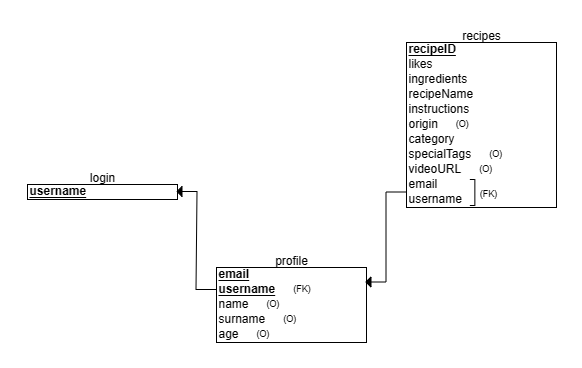
\includegraphics[width=1\linewidth]{slike/ERdiagram.png}
			    \caption{Dijagram baze podataka}
			    \label{fig:enter-label}
			\end{figure}
			
			\eject
			
			
		\section{Dijagram razreda}
		
			\textit{Potrebno je priložiti dijagram razreda s pripadajućim opisom. Zbog preglednosti je moguće dijagram razlomiti na više njih, ali moraju biti grupirani prema sličnim razinama apstrakcije i srodnim funkcionalnostima.}\\
			
			\textbf{\textit{dio 1. revizije}}\\
			
			\textit{Prilikom prve predaje projekta, potrebno je priložiti potpuno razrađen dijagram razreda vezan uz \textbf{generičku funkcionalnost} sustava. Ostale funkcionalnosti trebaju biti idejno razrađene u dijagramu sa sljedećim komponentama: nazivi razreda, nazivi metoda i vrste pristupa metodama (npr. javni, zaštićeni), nazivi atributa razreda, veze i odnosi između razreda.}\\
			
			\textbf{\textit{dio 2. revizije}}\\			
			
			\textit{Prilikom druge predaje projekta dijagram razreda i opisi moraju odgovarati stvarnom stanju implementacije}
			
			
			
			\eject
		
		\section{Dijagram stanja}
			
			
			\textbf{\textit{dio 2. revizije}}\\
			
			\textit{Potrebno je priložiti dijagram stanja i opisati ga. Dovoljan je jedan dijagram stanja koji prikazuje \textbf{značajan dio funkcionalnosti} sustava. Na primjer, stanja korisničkog sučelja i tijek korištenja neke ključne funkcionalnosti jesu značajan dio sustava, a registracija i prijava nisu. }
			
			
			\eject 
		
		\section{Dijagram aktivnosti}
			
			\textbf{\textit{dio 2. revizije}}\\
			
			 \textit{Potrebno je priložiti dijagram aktivnosti s pripadajućim opisom. Dijagram aktivnosti treba prikazivati značajan dio sustava.}
			
			\eject
		\section{Dijagram komponenti}
		
			\textbf{\textit{dio 2. revizije}}\\
		
			 \textit{Potrebno je priložiti dijagram komponenti s pripadajućim opisom. Dijagram komponenti treba prikazivati strukturu cijele aplikacije.}
